\section{Introduction}

\begin{figure}[t]
  \centering
  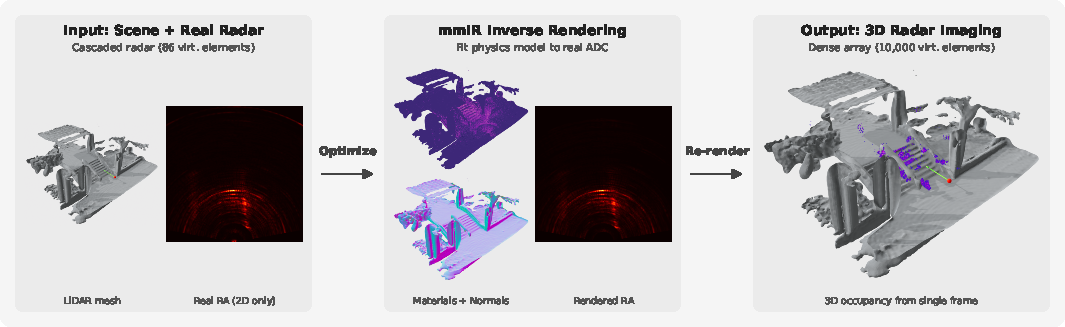
\includegraphics[width=\linewidth]{figs/teaser/teaser_v3.pdf}
  \caption{\textbf{Left:} LiDAR mesh and real 2D range--azimuth (RA) map from a commodity cascaded radar. \textbf{Center:} mmIR optimizes per-vertex materials, normals, and antenna beam patterns by fitting rendered ADC to real measurements. \textbf{Right:} The optimized scene is re-rendered from a dense 100$\times$100 virtual array for single-frame 3D occupancy detection.}
  \label{fig:teaser}
\end{figure}

Millimeter-wave (mmWave) radar penetrates fog, rain, and airborne dust~\cite{guan2020through}, measures Doppler velocity, and returns strong echoes from metals, yet it remains underutilized for 3D scene understanding. Commercial single-chip radars have only tens of antennas, limiting angular resolution to several degrees~\cite{gao2019experiments}, and their axis-biased layouts yield 2D range--azimuth (RA) slices rather than full 3D range--azimuth--elevation (RAE) volumes. Public datasets further limit access by providing only post-processed outputs (RA maps or sparse point clouds) rather than raw ADC~\cite{barnes2020oxford,caesar2020nuscenes}. The result is a shortage of high-resolution, 3D, raw FMCW ADC data: the fundamental bottleneck for learning-based radar perception. Detection, segmentation, occupancy prediction, and super-resolution all require training signal that current sensors and datasets cannot supply, and addressing this gap would enable these applications.

Existing approaches each fall short. Hardware scaling~\cite{sun2020mimo} increases cost without addressing data diversity. SAR~\cite{watts20162d,lin2023millimeter,zhang20173d} requires mechanical scanning impractical at fleet scale. Neural and Gaussian synthesis methods~\cite{mostajabi2020high,10.1145/3641519.3657510,huang2024dart,takawale2025spinr,kung2025radarsplat} are bottlenecked by the very data scarcity they aim to address: models trained on low-resolution 2D RA maps cannot recover 3D structure that was never observed.

Physics-based ray tracing (SBR) for mmWave is well established~\cite{dudek2010millimeter,sionna}, but existing pipelines are forward-only: geometry and materials must be specified \emph{a priori}, with no mechanism to calibrate against real measurements. Differentiable rendering has closed this gap for RGB~\cite{li2018differentiable, zhang2022iron}, LiDAR~\cite{kato2020differentiable}, and acoustics~\cite{jin2024diffsound}, and emerging RF methods take initial steps. Sionna RT~\cite{sionna} exposes gradients for antenna patterns and scattering coefficients but not through ray tracing itself (no geometry or normal gradients) and does not model wideband FMCW signals. Hofmann et al.~\cite{hofmann2025inverse} estimate SFCW materials but assume known geometry with single-bounce propagation, and InverTwin~\cite{chen2025invertwin} addresses multipath gradient pathologies but validates on synthetic data only. What is missing is an end-to-end differentiable FMCW renderer that can learn scene parameters from real radar captures without requiring ground-truth materials.

We present mmIR, an open-source differentiable FMCW radar inverse renderer that fits a physics-based forward model to real captures and re-renders from dense virtual apertures to synthesize high-resolution 3D radar data. Radar resolution is too coarse to reconstruct geometry directly, so we use LiDAR-derived meshes~\cite{kazhdan2006poisson} as a geometric scaffold, a practical choice given the far greater availability and resolution of LiDAR data. Inverse rendering then recovers the electromagnetic properties: mmIR optimizes per-vertex ITU physics materials (permittivity, roughness, correlation length, blend factor, slab thickness), vertex normals, and antenna beam patterns through end-to-end automatic differentiation of a phase-coherent MIMO forward model with multi-bounce propagation, polarization-aware BSDFs, specular manifold sampling~\cite{zeltner2020specular}, and free-space diffraction~\cite{steinberg2024fsd}. The pipeline also supports differentiable geometry and 6-DoF pose gradients with projective boundary sampling~\cite{zhang2023projective}, though we keep these fixed in our experiments because LiDAR-radar alignment preprocessing (Sec.~\ref{sec:supp_alignment} in the supplement) already provides accurate geometry and pose. After fitting, the optimized scene is frozen and re-rendered from arbitrarily large virtual apertures to synthesize dense, physics-consistent raw ADC (Fig.~\ref{fig:teaser}), enabling downstream applications such as 3D occupancy detection, radar super-resolution, and synthetic training data generation that would otherwise require prohibitively large physical arrays.

On seven outdoor ColoRadar~\cite{kramer2022coloradar} scenes, mmIR achieves 0.63 mean Pearson RA correlation versus 0.32 for Sionna-RT. We demonstrate cross-sensor transfer: scenes trained on a cascaded imaging radar (12TX$\times$16RX, 86 virtual elements) produce valid ADC for a co-located single-chip radar (3TX$\times$4RX, 12 virtual elements) without re-training (0.58 correlation), providing evidence that the optimized scenes capture transferable physics rather than sensor-specific patterns. We further show single-frame 3D occupancy detection from dense virtual arrays (100TX$\times$100RX) validated against LiDAR. Our contributions are:

\begin{enumerate}
\item To the best of our knowledge, the first open-source, end-to-end differentiable inverse renderer for wideband FMCW radar, enabling joint optimization of per-vertex materials, normals, and antenna patterns directly from real radar captures, with support for multi-bounce propagation, specular manifold sampling, polarization-aware BSDFs, free-space diffraction, and differentiable geometry and pose gradients with projective boundary sampling.
\item A virtual-aperture re-rendering framework that synthesizes high-resolution 3D raw ADC from fitted scenes via arbitrarily large synthetic arrays, enabling 2D-to-3D lifting and 3D occupancy detection.
\item Cross-sensor transfer validation on real COTS radar, demonstrating that scenes optimized on one sensor generalize to a different configuration without re-training.
\end{enumerate}

\subsection{Scope}
\label{sec:scope}

The primary goal of mmIR is high-quality ADC radar data synthesis: by fitting a differentiable forward model to real radar captures on real LiDAR-derived geometry, mmIR produces dense, physics-consistent raw ADC that would otherwise require expensive hardware arrays to acquire. We envision practitioners using optimized scenes to generate large-scale datasets for training downstream perception models (detection, segmentation, occupancy prediction) without additional data collection. We validate on real measurements from commercial off-the-shelf (COTS) radars, specifically the Texas Instruments MMWCAS-RF-EVM cascade and AWR1843 single-chip sensors, demonstrate cross-sensor transfer, and show that the synthesized data is sufficient for single-frame 3D occupancy detection from dense virtual arrays (Sec.~\ref{sec:3d_occupancy}). Our experimental evaluation compares against open-source, physics-based ray-tracing inverse rendering methods (Table~\ref{tab:polarization_comparison}), ensuring reproducibility and a like-for-like comparison of explicit forward models.
